\documentclass[11pt]{article}
\usepackage{enumitem}
\usepackage{amsmath}
\usepackage{bbm}
\usepackage{graphicx}
\usepackage{caption}
\usepackage{verbatim}
\usepackage{subcaption}
\usepackage{mdframed}
\usepackage{fancyhdr}
\usepackage{tikz}
\usepackage{tikz-qtree}
\usepackage{hyperref}
\usepackage{algorithm}
\usepackage{algpseudocode}
\usepackage{pdfpages}
\pagestyle{fancy}
\lhead{Killian Rutherford (KRR2125) \\
Richard Godden (RG3047)}
\rhead{COMS 4111 Project 1.1}
\renewcommand{\headrulewidth}{0.4pt}
\renewcommand{\footrulewidth}{0.4pt}

\begin{document}

\center{\section*{Tennis Singles Tournament Database}}

\begin{mdframed}
\center{\textbf{Approved By Aayush Mudgal}}
\end{mdframed}


\hfill \break
\raggedright\subsection*{Paragraph}

\begin{enumerate}

\item The database will be storing information for singles tennis tournaments, in the point of view of a tournament organiser/data provider. There will be seven entities (revised from the original 6 we brought to the meeting): Tournaments, Players, Matches, Courts, Spectators, Tickets and the newly added Complex. The organisation aspect will involve court numbers/tickets and spectators, whilst data provided will be relevant to player and match stats. Users will be able to query this database to discover player stats and match outcomes (E.g. who won which match, what those match statistics were, what the player statistics in the tournament were, what their overall statistics are, etc..). As well as looking at logistics, enquiries about where the matches are taking place, ticket prices, and spectator statistics. Challenges will involve the large number of features we will have to include in this database, as well as looking at the relationships between the entity sets. Some are not so obvious, particularly with the tickets (can be different types), not necessarily one to one relationships (1 ticket may not be to 1 match) and name changes etc. For now we have restricted this condition to one match per ticket which, we may change in the future.

After meeting with the TA, we made the following revisions:
\begin{enumerate}[label = (\alph*)]
\item We incorporated a few more real-world constraints (see below)
\item We modified our E-R diagram as we initially had too many complex attributes for each set
\item We changed relationships between sets (in matches v. players case)
\item We modified our SQL schema so that we did not necessarily have one table for each relational set. In the 1-1 and 1-many cases we just included a foreign key within the respective entity table 
\end{enumerate}

We have factored in real-world constraints throughout. The most predominant examples are our SQL constraints, such as ensuring there is a unique winner for each match. Further, a match can have multiple start times, which would indicate a suspension (and may end up being played on different courts). In the examples of tickets, we are also distinguishing buyers from reserved for, as 1 person can buy multiple tickets for others. Many more of real world relationships can be observed on our E-R diagram.

We will be choosing the Web Front-End Option for Part 3 (Option 3.a).

We will fill all the player and match data with real data from Jeff Sackmann tennis$\_$atp github $(https://github.com/JeffSackmann/tennis\_atp)$. The spectator and ticket details may require further research $/$fill in fake data.
\end{enumerate}


\subsection*{Contingency Plan}
We do not anticipate needing this, but our contingency plan would simply be to take out the Tickets and Spectators entity sets, and simply deal with Players, Matches, Complex, Courts and Tournaments. After our meeting, the TA told us we could even further eliminate one of the sets Courts or Complex if need be.

\newpage
\subsection*{E-R Diagram}
\includegraphics[width=1.3\textwidth, angle = -90]{ER_tennis_database.png}

\newpage
\subsection*{SQL Schema}
\verbatiminput{SQL_SCHEMA.txt}

\newpage
\subsection*{Copy of Proposal approved by TA}
\begin{mdframed}
\center{\textbf{Approved By Aayush Mudgal}}
\end{mdframed}

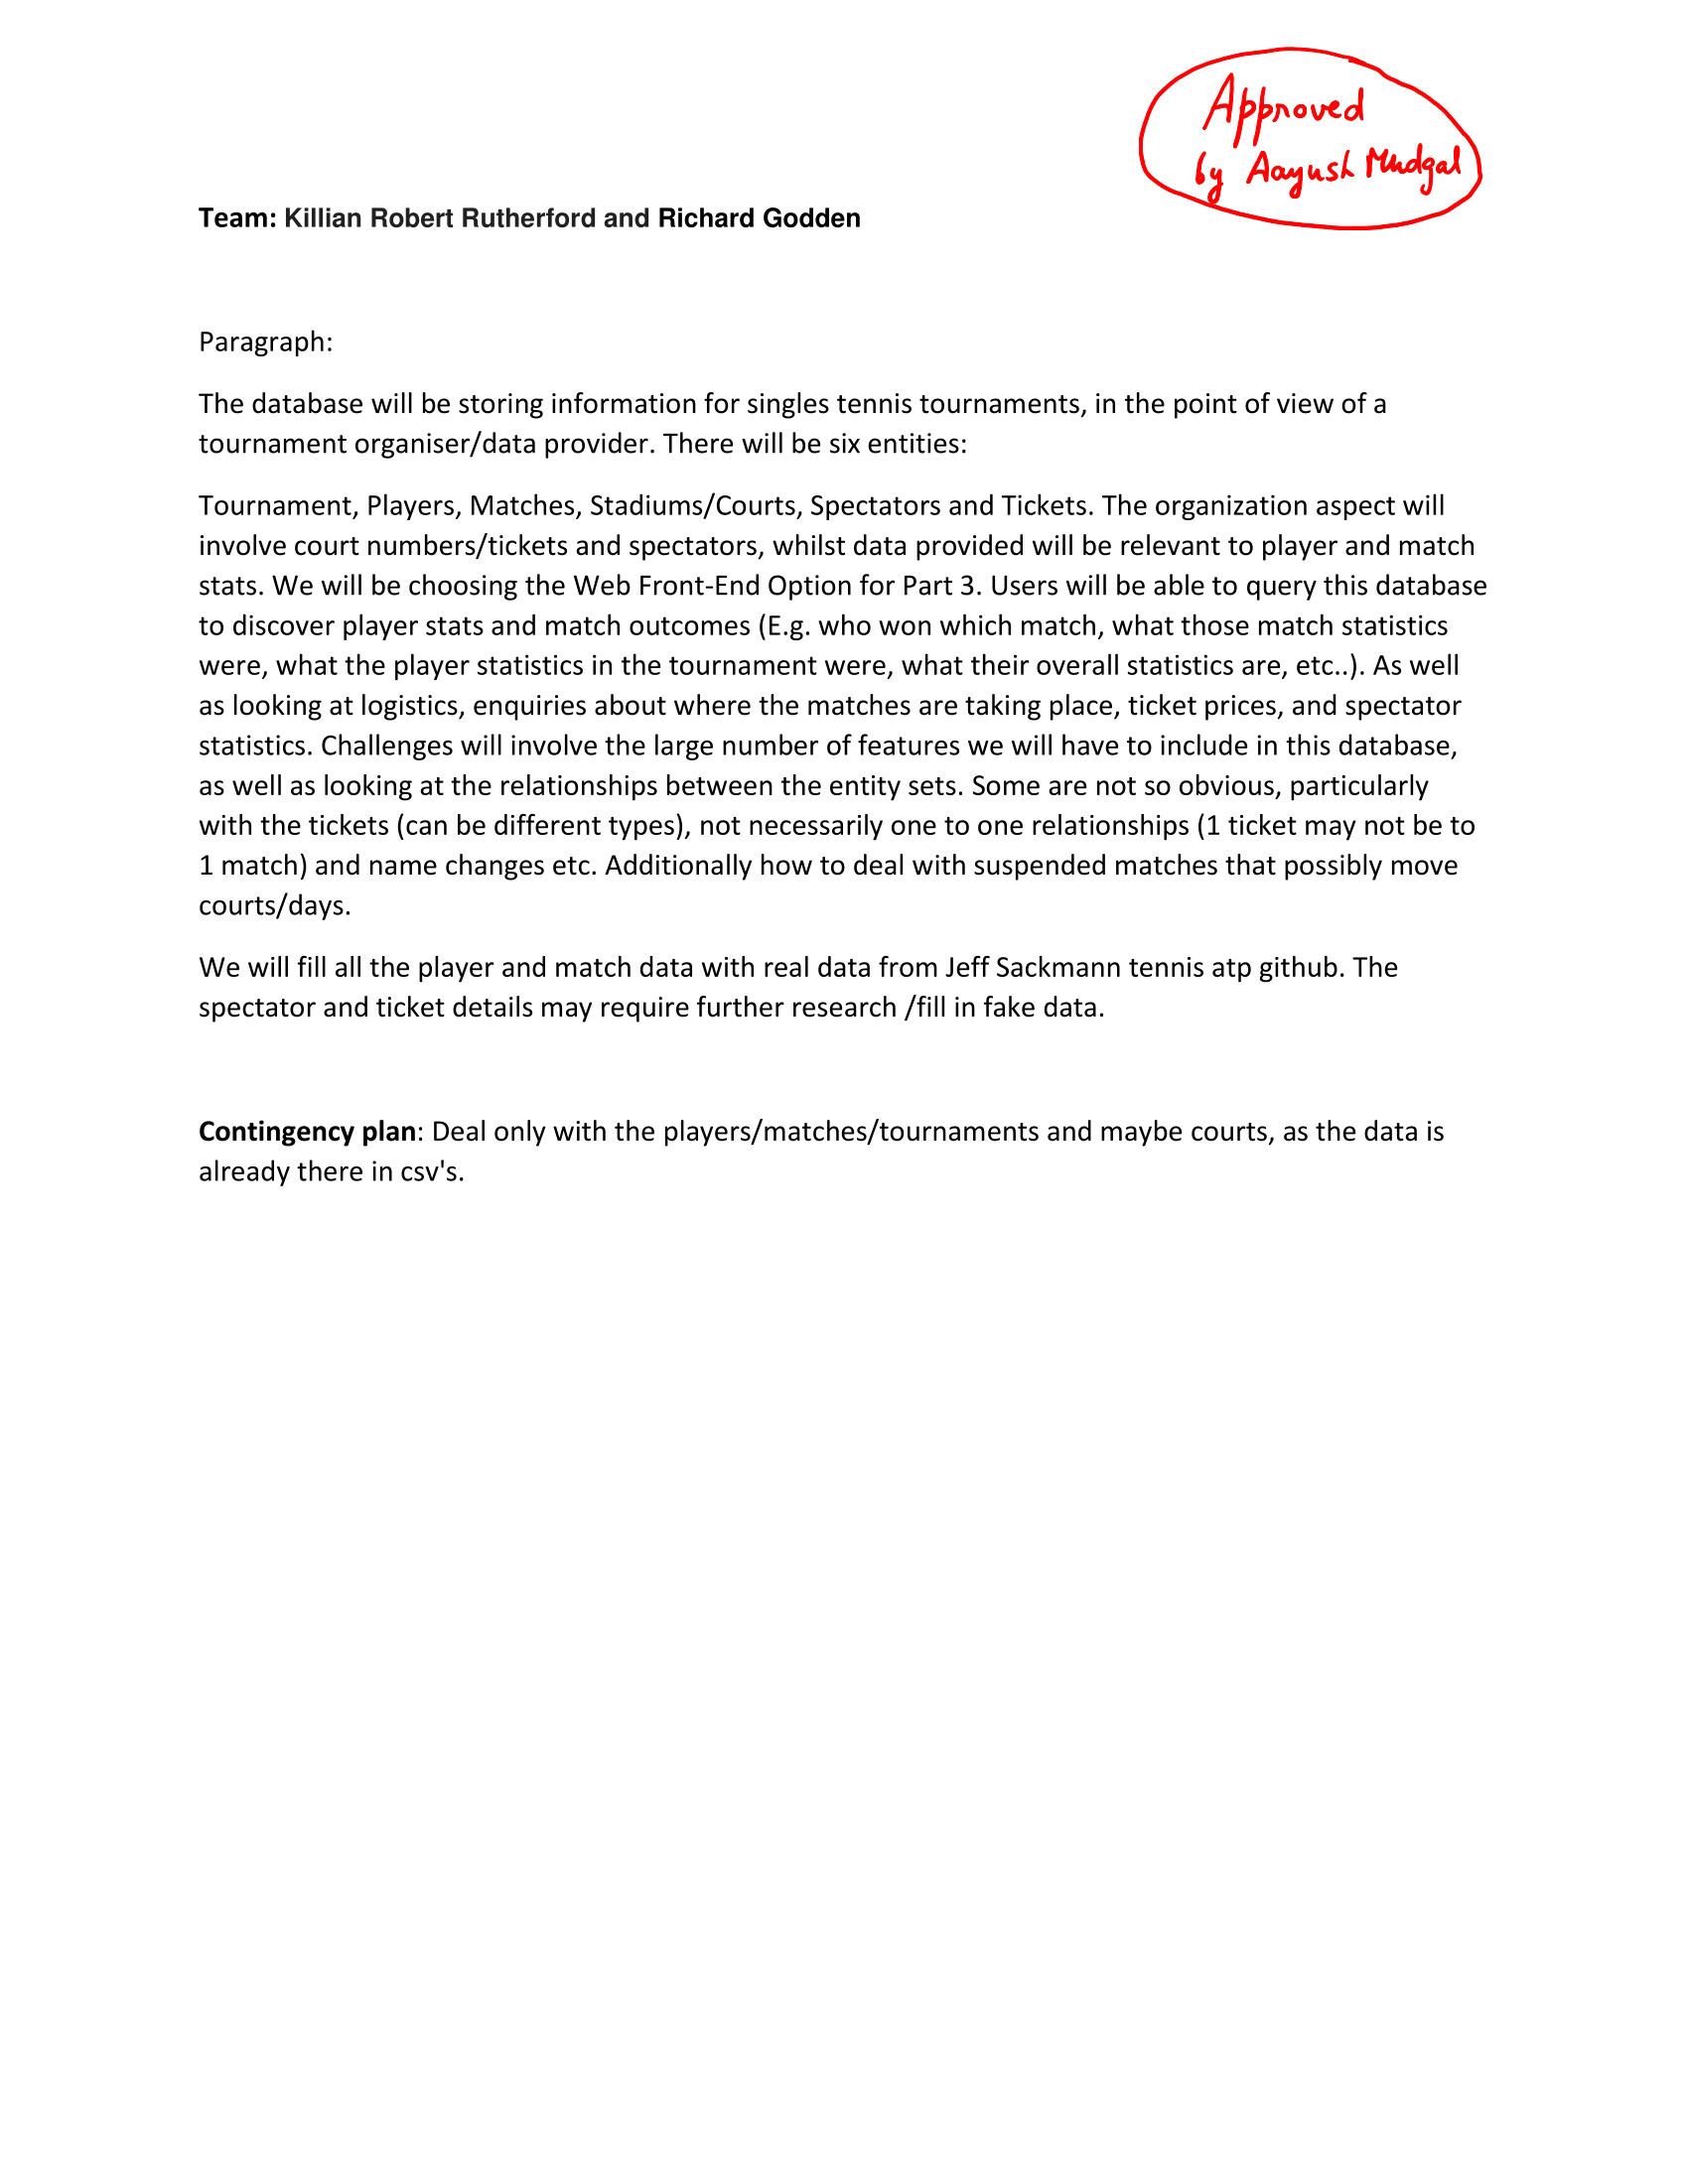
\includegraphics[width=1\textwidth]{killian_richard-1.png}




\end{document}